\section{Rešitev + Dodatna naloga}

Poglejmo si najprej točno integrirani rešitvi za oba primera
\begin{figure}[h]
    \centering
    \includegraphics[width=10cm]{pdfs/ress.pdf}
    \caption{Točno integrirane rešitve diferencialne enačbe, s parametrom $k=0.1$, $T_{zun}=0$ in $A = 10$ }
\end{figure}

Potem si še poglejmo hitrost različnih algoritmov.
\begin{figure}[h]
    \centering
    \includegraphics[width=11cm]{pdfs/cas.pdf}
    \caption{Časovna odvisnost algoritmov}
\end{figure}
Vidimo, da se algoritem \verb|rkf| vede konstantno. In tudi se, ker ni vezan
na evaluacijo danih točk, le dolžino intervala in tolarance.
\newpage
Sedaj si poglejmo, kako se algoritmi za prvo diferencialno enačbo vedejo, če spreminjamo parametre.
\begin{figure}[h]
    \centering
    \includegraphics[width=8cm]{pdfs/T(t,k).pdf}
    \includegraphics[width=8cm]{pdfs/T(t,k)_log.pdf}

    \caption{Rešiteve diferencialne enačbe $T'(t) = -k(T-T_{zun})$, če spreminjamo k}
\end{figure}
Poglejmo si še kaj se dogaja pri drugi diferencialni enačbi.
\begin{figure}[h]
    \centering
    \includegraphics[width=8cm]{pdfs/T1(t,k).pdf}
    \includegraphics[width=8cm]{pdfs/T1(t,k)_log.pdf}

    \caption{Rešiteve diferencialne enačbe $T'(t) = -k(T-T_{zun}) + A\sin(2\pi t)$, če spreminjamo k}
\end{figure}
\newpage
Poglejmo si še kaj se dogaja z algoritmomi knjižnjice \verb|scipy.solve_ivp()|, če se ne dotikamo ne absolutne 
ne relativne tolerance.

\begin{figure}[h]
    \centering
    \begin{subfigure}[b]{0.45\textwidth}
        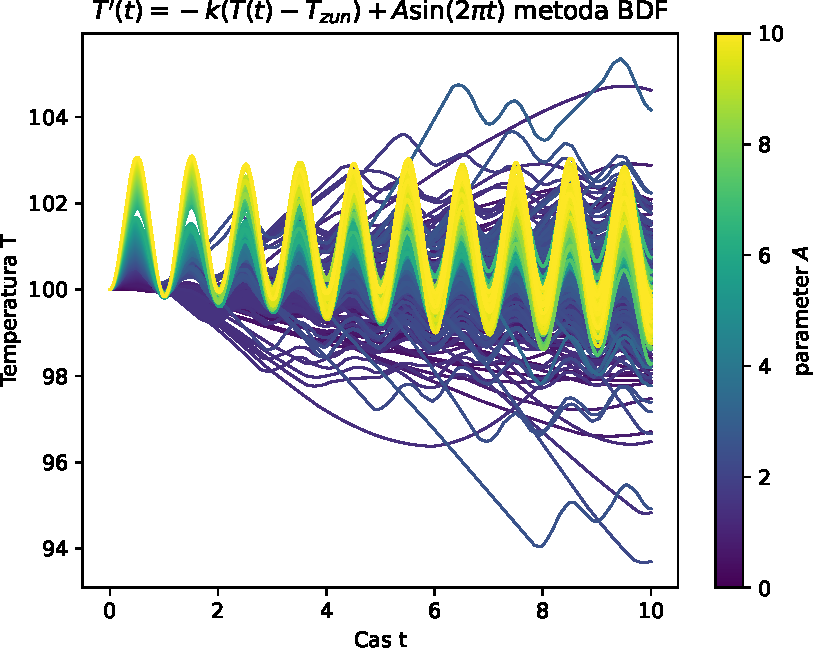
\includegraphics[width=\textwidth]{pdfs/A_BDF.pdf}
    \end{subfigure}
    \hfill
    \begin{subfigure}[b]{0.45\textwidth}
        \includegraphics[width=\textwidth]{pdfs/A_DOP853.pdf}
    \end{subfigure}
    \par
    \begin{subfigure}[b]{0.45\textwidth}
        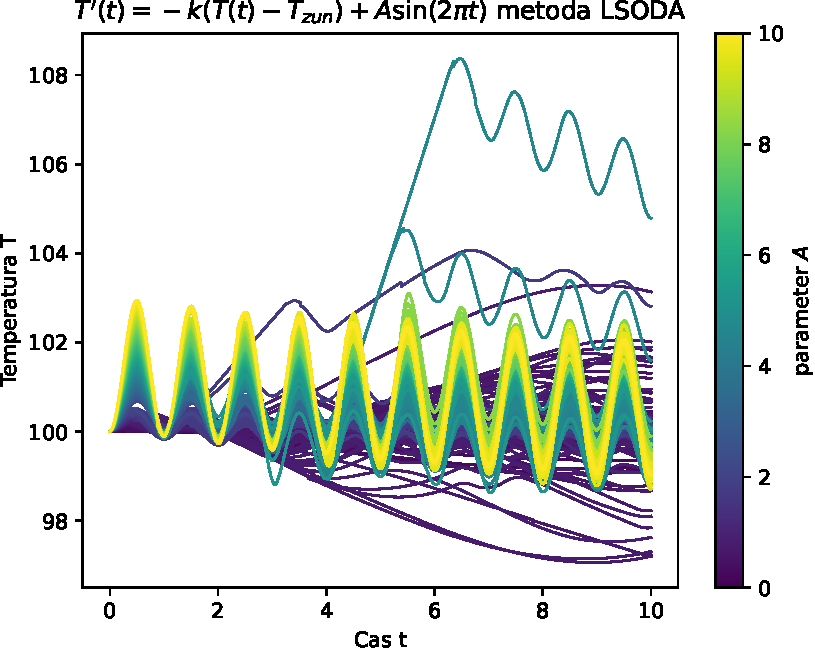
\includegraphics[width=\textwidth]{pdfs/A_LSODA.pdf}
    \end{subfigure}
    \hfill
    \begin{subfigure}[b]{0.45\textwidth}
        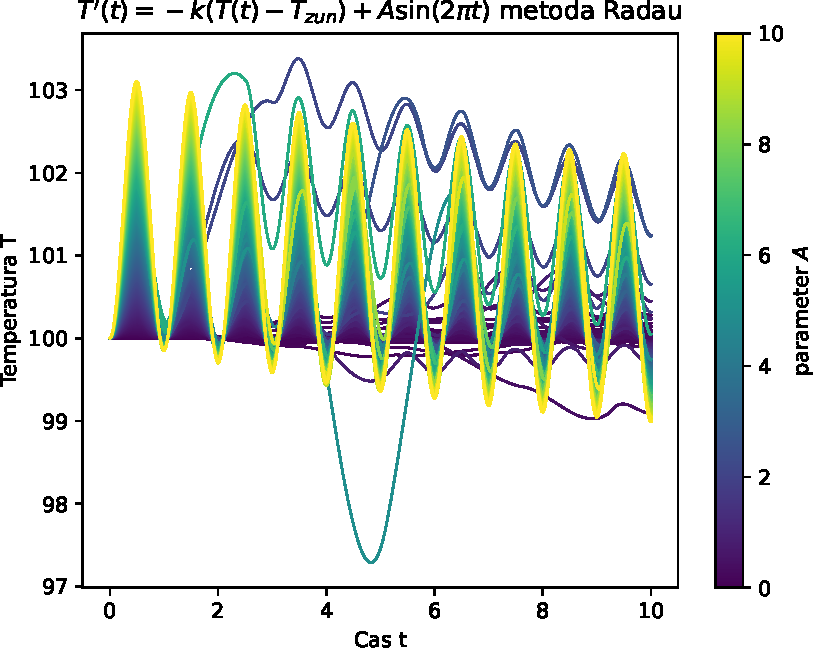
\includegraphics[width=\textwidth]{pdfs/A_Radau.pdf}
    \end{subfigure}
    \par
    \begin{subfigure}[b]{0.45\textwidth}
        \includegraphics[width=\textwidth]{pdfs/A_RK23.pdf}
    \end{subfigure}
    \hfill
    \begin{subfigure}[b]{0.45\textwidth}
        \includegraphics[width=\textwidth]{pdfs/A_RK45.pdf}
    \end{subfigure}
    \caption{Rezultati različnih algoritmov z istimi parametri, brez nastavljanja tolerance}
\end{figure}

\newpage
\begin{figure}[h]{}
    \centering
    \includegraphics[width=12cm]{pdfs/A_tocna.pdf}
    \caption{Točna rešitev, z zelo nizko toleranco}
\end{figure}
\newpage
